\documentclass[11pt]{article}
\usepackage[a4paper, left=0.75in, right=0.75in, top=0.5in, bottom=0.5in]{geometry}
\usepackage{amsmath, bm}
\usepackage{amssymb}
\usepackage{solarized-light}
\usepackage{hyperref}
\hypersetup{
    colorlinks=true,
    linkcolor=blue,
    filecolor=magenta,      
    urlcolor=blue,
}
\usepackage{graphicx}
\graphicspath{ {.} }

\title{ES 404 - Midsem Examination}
\date{}
\author{Nishant Tatar - 21110223}

\begin{document}
\maketitle

For Questions 1 to 6, the python code has been uploaded to a \href{https://colab.research.google.com/drive/13LGfweQzj7sSejKYgvT02PPBfOn1-AWh?usp=sharing}{Colab Notebook}. Since I was reading from a file, and the files did not persist between instances, I have used urls to the csv files on my github.

\section{Network Visualisation}
For this, I used cartopy library for plotting the network onto a real world graph. Coordinates were taken from Google's Developer Public Data portal.

\begin{figure}[h]
    \centering
    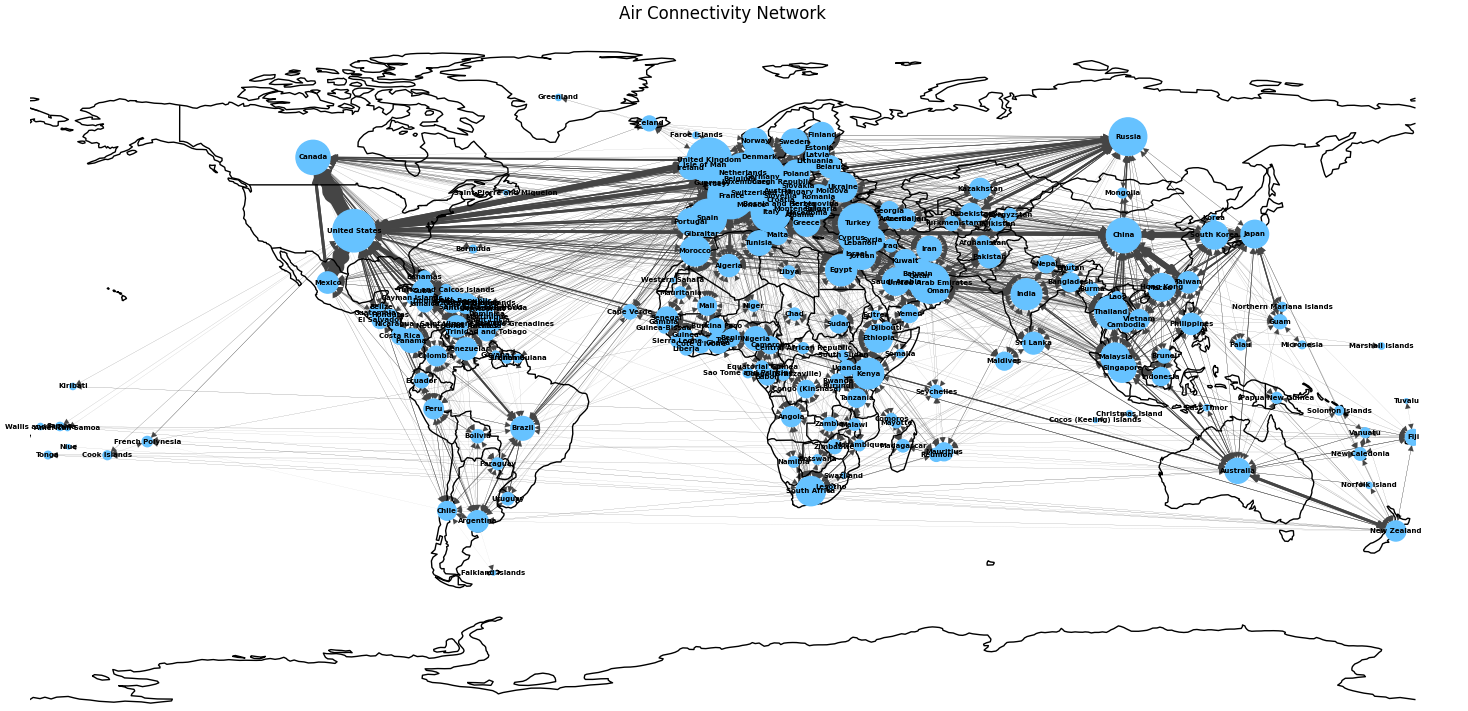
\includegraphics[width=0.75\textwidth]{geocodenetwork.png} % Replace example-image with the filename of your image
    \caption{Air Connectivity Network}
\end{figure}

\section{Degree Distibution Plotting and Characterisation}
\subsection{Degree Distribution plotting}
Applying Lograithmic Binning on the degree distribution.
\begin{figure}[h]
    \centering
    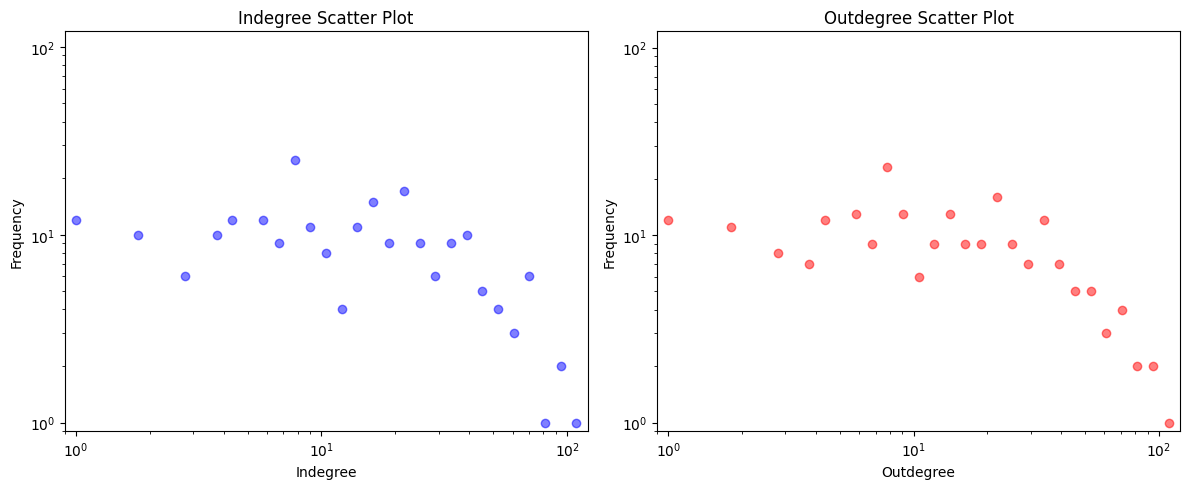
\includegraphics[width=0.75\textwidth]{logbinneddegplot.png} % Replace example-image with the filename of your image
    \caption{Logarithmic Binning}
\end{figure}

\subsection{Distribution Characterisation}
I applied two Goodness of Fit tests on the given degree distribution, KS and Cramer Von Mises test, and then found the p value for the out degree and in degree distributions. I took nearly all continuous distributions from scipy.stats module, and applied KS and CVM goodness of fit tests. For all distributions with a p value $<$ 0.05, I discarded those distributions. \\
The following distributions had a p value greater than 0.05 for both KS and CVM tests: fatiguelife, fisk, foldcauchy, genextreme, genpareto, gibrat, gompertz, halfcauchy, halfgennorm, invgamma, invgauss, invweibull, johnsonsb, johnsonsu, kappa3, lognorm, lomax, nct, norminvgauss, pareto, powerlognorm, recipinvgauss, skewcauchy, truncpareto, wald. \\
While none of these distributions cannot be ruled out, the highest p value for the CVM test was fatiguelife, and as such, the degree distribution is most similar to \textbf{fatiguelife} as compared to all other distributions.
\section{Pearson Coefficient}
The Pearson correlation coefficient, denoted as $r$, is a measure of the linear correlation between two distributions. It ranges from -1 to 1, where:
\begin{itemize}
    \item $r = 1$ indicates a perfect positive linear relationship,
    \item $r = -1$ indicates a perfect negative linear relationship,
    \item $r = 0$ indicates no linear relationship between the variables.
\end{itemize}

The formula to calculate the Pearson correlation coefficient between two distributions $x$ and $y$ with $n$ data points is:
$$ r = \frac{{\sum_{i=1}^{n} (x_i - \bar{x})(y_i - \bar{y})}}{{\sqrt{\sum_{i=1}^{n} (x_i - \bar{x})^2} \sqrt{\sum_{i=1}^{n} (y_i - \bar{y})^2}}} $$

Where $x_i$ and $y_i$ are the individual data points, $\bar{x}$ and $\bar{y}$ are the means of the $x$ and $y$ distributions respectively.
\subsection{Degree and Betweenness Centrality}
The Pearson Coefficient between the Degree and Betweenness Centralities for the network is $0.7368$.
\subsection{Degree and Closeness Centrality}
The Pearson Coefficient between the Degree and Closeness Centralities for the network is $0.9006$.
\subsection{Eigenvector and Degree Centrality}
The Pearson Coefficient between the Eigenvector and Degree Centralities for the network is $0.9604$.
\section{Degree Centrality and Strength of Node}
The Degree Centrality is the number of nodes that are connected to a particular node, and the Strength of a node refers to the sum of the weights incident on the node.
\begin{center}
    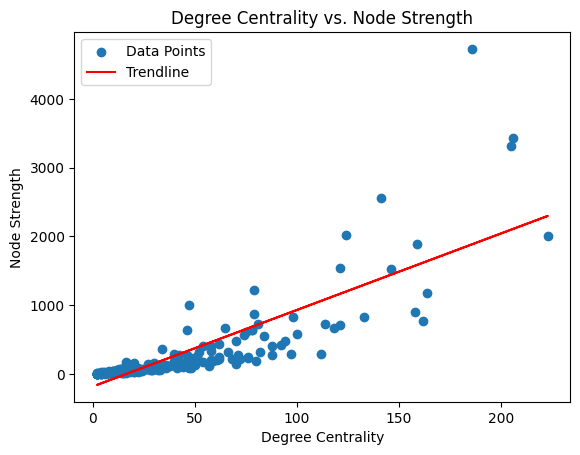
\includegraphics[scale=0.5]{degcent.png}\\
    Linear Correlation Coefficient $(r) = 0.82154$ 
\end{center}

\section{Degree vs Clustering Coefficient}
\begin{center}
    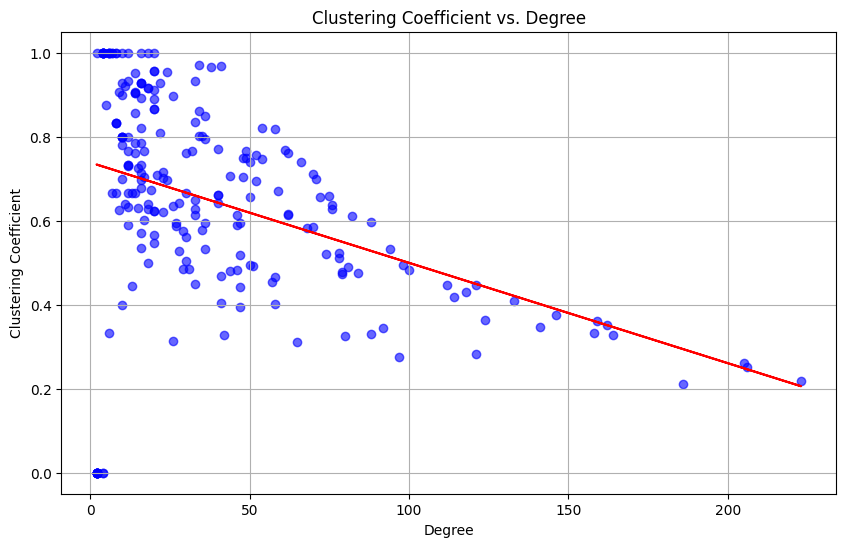
\includegraphics[scale=0.6]{ccvd.png}\\
    Linear Correlation Coefficient $(r) = -0.383121$ 
\end{center}
As such, as the value of r is negative, the clustering coefficient of the node goes down.
\section{Small World vs Ultra Small World}
The average shortest path is calculated using python. The number of nodes in the airport network are 227. Calculating the log and comparing it to the average shortest path, we find that the network is a small world network, as the average shortest path $\approx \log{N}$
\pagebreak
\section{Clustering Coefficients BA and ER Networks}
The Local Clustering Coefficient is a measure of how close the neighbors of a node are to forming a complete clique. This is a measure of network connectivity, and is defined as $C_i = \frac{2 \times (T_i)}{(k_i) \times (k_i - 1)} $ . Where $T_i$ is the number of triangles passing through the node i and $k_i$ is the degree of node $i$. Another Way to look at this could be as the ratio of realised connections compared to number of possible connections.

\subsection{Barabasi Albert Model}
For the Barabasi Albert Model, where one node appears one at a time with $m$ edges ready to connect to the network for a particular node, it connects to existing nodes in the network with a probability proportional to their degrees.\\
At time when node i arrived, we assume that node j was already present. 
$$k_j (i) = \left( \frac{i}{j} \right) ^ {1/2} $$
The probability that i would connect with j is:
$$P_{i,j} = \frac{m \times k_j (i)}{2 \times m \times i} = \frac{m}{2 \sqrt{i j}}$$
Similarly for $P_{j,l}$ and $P_{l,i}$, we get $\frac{m}{2 \sqrt{j l}}$ and $\frac{m}{2 \sqrt{l i}}$. \\
Hence, the Local Clustering Coefficient is:
$$C_l = \frac{2 \int_{i=l,i>j}^{N-1} di \int_{j=1}^{N-1} P_{i,j} P_{j,l} P_{l,i} \, dj}{(k_l) \cdot (k_l - 1)}$$
The Entire Integrand can be shown as:
$$2 \int_{i=l,i>j}^{N-1} di \int_{j=1}^{N-1} P_{i,j} P_{j,l} P_{l,i} \, dj= \frac{m^3}{8} \int \int \left[ \frac{1}{\sqrt{ij}} \cdot \frac{1}{jl} \cdot \frac{1}{li}\right] di dj$$
$$ = \frac{m^3}{8l} \int \int \left(\frac{1}{i}\cdot\frac{1}{j}\right) di dj$$
$$ = \frac{m^3}{8l} \left| \ln{i} \right| _{i=1, i>j}^{N-1} \left| \ln{j} \right| _{j=1}^{N-1}$$
$$ \approx \frac{m^3}{8l} \left( \ln{N}\right)^2$$ 
Therefore, $C_l$ is:
$$C_l = \frac{2\cdot\frac{m^3}{8}\left( \ln{N}\right)^2}{(k_l) \cdot (k_l - 1)}$$
and $$ k_l = m \cdot \left( \frac{N}{l}\right)^{1/2}$$
For sufficiently large N, the equation reduces to:
$$ C_l = \frac{m}{4} \cdot \frac{\left( \ln{N}\right)^2}{N} $$

\subsection{Erdos Renyi Model}
We define $C_i$ as $ \frac{2 \cdot T_i}{(k_i)\cdot(k_i - 1)}$,  where $T_i$ is the number of triangles passing through node i, or, the expected number of edges between the neighbors of the node. In an ER network with $ N $ nodes and edge probability $ p $, the expected number of edges connected to node $ i $, denoted as $ k_i $, follows a binomial distribution with parameters $ N-1 $  and $ p $. So, $ k_i = (N-1)p $. \\ \\
\textbf{The expected value of $T_i$ is determined as follows:}\\
Since edges between pairs of nodes are independent, the expected number of edges between the neighbors of node $ i $ is the probability that a pair of neighbors is connected, multiplied by the total number of possible pairs of neighbors. Each neighbor of node $ i $ has $ k_i $ possible connections, and the probability that any particular pair of them is connected is $ p $.\\
As such, expected number of edges for node $i$ is:
$$ T_i = \frac{k_i(k_i-1)}{2} \times p $$ \\
Plugging this back into the equation for $ C_i $:

$$ C_i = \frac{2 \times \frac{k_i(k_i-1)}{2} \times p}{k_i(k_i-1)} $$
$$ C_i = p $$

\section{Emergence of Scalefree nature in BA Model}
The Barabási–Albert (BA) model is characterized by a power-law distribution of node degrees, where the degree distribution follows a power-law function. Two essential requirements for the emergence of scale-free properties in the BA model are:

\begin{enumerate}
    \item \textbf{Preferential Attachment:}
    
    The first essential requirement is the principle of preferential attachment, where new nodes are more likely to connect to existing nodes that already have a high degree. 
    
    Mathematically, the probability $\Pi$ that a new node attaches to an existing node $i$ with degree $k_i$ is formulated as:
    $$ \Pi(k_i) = \frac{k_i}{\sum_j k_j} $$
    where $k_i$ represents the degree of node $i$, and $\sum_j k_j$ represents the sum of degrees of all nodes in the network. Here, a node that has higher degree is much more likely to have a node connect to it.

    \item \textbf{Network Growth:}
    
    The second essential requirement is that the network must grow. In the BA model, at each time step, a new node is added to the network, and it forms connections with existing nodes according to the preferential attachment rule. This continuous growth process, combined with preferential attachment, leads to the emergence of scale-free properties in the network, where the degree distribution follows a power-law.
\end{enumerate}

In summary, the combination of preferential attachment and continuous growth in the BA model drives the emergence of scale-free properties in complex networks. Preferential attachment biases the attachment of new nodes towards high-degree nodes, while the growth mechanism ensures the continuous expansion of the network, resulting in a power-law distribution of node degrees.

\pagebreak
\nocite{*} % Include all entries from the bibliography file

\bibliographystyle{ieeetr}
\bibliography{references}

\end{document}